\chapter{Volatilidade: ARCH e GARCH}
\label{cap:garch}

\section{O problema}
Retornos financeiros têm três traços estáveis: (i) quase sem autocorrelação, (ii) \emph{quadrados} dos retornos fortemente autocorrelacionados (a volatilidade vem em ondas: calmaria, turbulência), (iii) caudas mais pesadas do que as de uma normal. Um ARMA clássico supõe variância constante e não captura nada disso.

\section{ARCH(1) e GARCH(1,1)}
Escreva o retorno (já sem média) como $r_t=\sigma_t z_t$, com $z_t$ i.i.d. de média 0 e variância 1. No \textbf{GARCH(1,1)}:
\[
\sigma_t^2=\omega+\alpha\,r_{t-1}^2+\beta\,\sigma_{t-1}^2,\qquad \omega>0,\ \alpha,\beta\ge0.
\]
\begin{itemize}[leftmargin=1.4em]
\item O ARCH(1) é o caso $\beta=0$: a volatilidade de hoje depende só do choque de ontem.
\item \textbf{Estacionariedade}: $\alpha+\beta<1$. Variância incondicional: $\omega/(1-\alpha-\beta)$.
\item $\alpha+\beta$ mede a \textbf{persistência}. Valores próximos de 1 (como 0{,}97) são típicos em dados reais.
\item A curtose (de $r_t$) é maior do que 3 mesmo com $z_t$ normal.
\end{itemize}

\begin{simulacao}[{Conferido por simulação}]
Com $\omega=0{,}1$, $\alpha=0{,}1$, $\beta=0{,}85$ e uma simulação longa (400 mil pontos): variância $2{,}009$ (teoria: $0{,}1/0{,}05=2$); curtose $3{,}774$ (teoria: $3{,}774$); autocorrelação de $r_t^2$ no lag 1: $0{,}177$ (teoria: $0{,}179$). A autocorrelação de $r_t$ ficou próxima de zero ($0{,}04$ numa amostra de 2000 pontos), mas a de $r_t^2$ foi $0{,}15$. Ruído branco nos retornos, dependência forte na volatilidade.
\end{simulacao}

\begin{center}
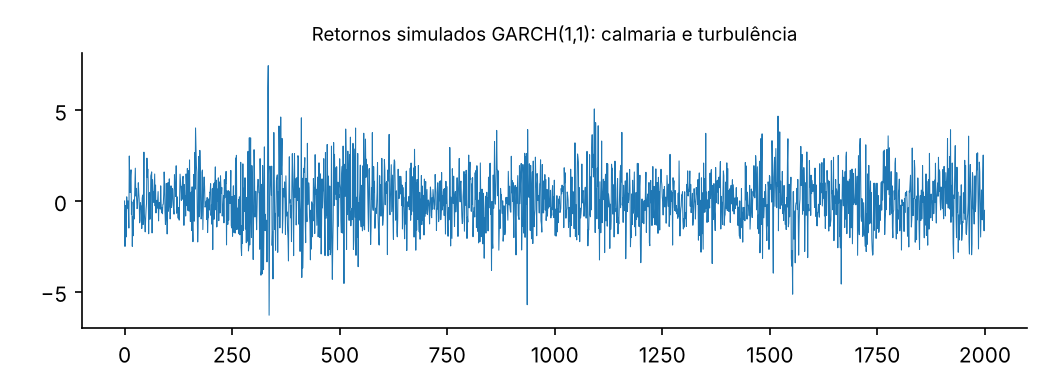
\includegraphics[width=0.9\textwidth]{fig/garch.png}
\end{center}

\begin{simulacao}[{Estimação: parâmetros individuais são difíceis}]
Ajustando um GARCH(1,1) a 2000 pontos simulados, obtive $\hat\omega=0{,}054$, $\hat\alpha=0{,}086$ e $\hat\beta=0{,}890$, contra os verdadeiros $0{,}1$; $0{,}1$; $0{,}85$. Os parâmetros individuais erraram bastante, mas a combinação que importa ficou próxima: persistência estimada $0{,}976$ (verdadeira $0{,}95$) e variância incondicional $0{,}054/0{,}024\approx2{,}26$ (verdadeira $2{,}0$). Em modelos muito persistentes, $\omega$, $\alpha$ e $\beta$ ficam fortemente correlacionados na estimação.
\end{simulacao}

\begin{atencao}
\begin{itemize}[leftmargin=1.2em]
\item \textbf{Não aplique ARCH a uma série com raiz unitária ou tendência}; trabalhe com retornos (diferenças de logaritmos).
\item \textbf{O GARCH simétrico não distingue notícias boas de ruins.} Para o efeito alavancagem (quedas aumentam mais a volatilidade do que altas), use GJR-GARCH ou EGARCH.
\item \textbf{Escolher $z_t$ normal subestima caudas}; muitos usam $t$ de Student.
\end{itemize}
\end{atencao}

\begin{exercicio}
GARCH(1,1) com $\omega=0{,}2$, $\alpha=0{,}1$, $\beta=0{,}8$. Calcule a variância incondicional e a previsão de $\sigma^2_{t+1}$ dado $r_t^2=4$ e $\sigma_t^2=3$.
\end{exercicio}
\sol{Variância incondicional: $0{,}2/(1-0{,}9)=2$. Previsão: $\sigma^2_{t+1}=0{,}2+0{,}1\times4+0{,}8\times3=0{,}2+0{,}4+2{,}4=3{,}0$.}

\begin{exercicio}
Por que $\alpha+\beta=1$ cria problemas, e como se chama esse caso?
\end{exercicio}
\sol{Com $\alpha+\beta=1$ a variância incondicional não existe (o denominador é zero) e choques de volatilidade nunca se dissipam. É o IGARCH. A previsão da volatilidade futura deixa de reverter para uma média de longo prazo.}
